\documentclass[11pt, a4paper]{article}
\usepackage[utf8]{inputenc}
\usepackage[greek,english]{babel}
\usepackage{alphabeta}
\usepackage{fontspec}
\usepackage{amsmath, amssymb, amsfonts}
\usepackage{graphicx}
\usepackage{geometry}
\usepackage{subcaption}
\usepackage{float}
\usepackage{listings}
\usepackage{xcolor}

\geometry{margin=1in}
\setmainfont{Times New Roman}

\title{Telecommunication Systems I \\ Exercise 2}
\author{Antonios Moutsopoulos AM:2021030024}
\date{April 27, 2026}

\begin{document}

\maketitle
\begin{center}
    Total number of hours: 2 hours
\end{center}

\section*{Part A: Baseband PAM waveforms}

\subsection*{A.1 SRRC Pulse and ESD}
We constructed an SRRC pulse $\phi(t)$ with $T=10^{-3}$, $over=10$, $A=4$, and $\alpha=0.5$. The Energy Spectral Density (ESD) was computed using the FFT.

\begin{figure}[H]
    \centering
    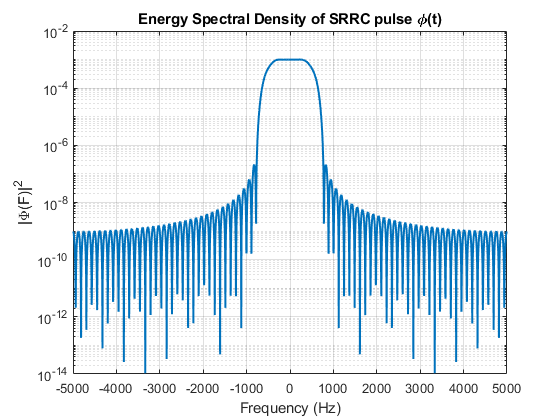
\includegraphics[width=0.7\textwidth]{A1.png}
    \caption{Energy Spectral Density $|\Phi(F)|^2$ of the SRRC pulse.}
    \label{fig:a1_esd}
\end{figure}

\subsection*{A.3 2-PAM PSD Estimation}
Using $N=100$ bits and $K=500$ realizations, we estimated the Power Spectral Density of the 2-PAM signal. The experimental result closely follows the theoretical curve $S_X(F) = \frac{\sigma_X^2}{T} |\Phi(F)|^2$, where $\sigma_X^2 = 1$.

\begin{figure}[H]
    \centering
    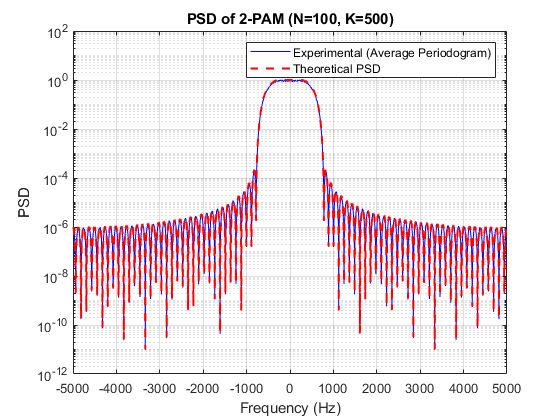
\includegraphics[width=0.7\textwidth]{A3.png}
    \caption{Experimental vs. Theoretical PSD for 2-PAM.}
    \label{fig:a3_psd}
\end{figure}

\textbf{Observation:} As $K$ and $N$ increase, the periodogram average becomes smoother and more accurate, providing a better approximation of the theoretical PSD.

\subsection*{A.4 4-PAM PSD Estimation}
For 4-PAM, we mapped bit pairs to symbols $\{+3, +1, -1, -3\}$. The variance is $\sigma_X^2 = 5$.

\begin{figure}[H]
    \centering
    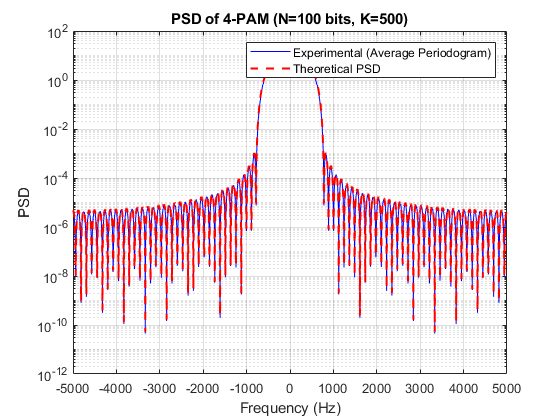
\includegraphics[width=0.7\textwidth]{A4.png}
    \caption{Experimental vs. Theoretical PSD for 4-PAM.}
    \label{fig:a4_psd}
\end{figure}

\textbf{Comparison:} The bandwidth of 4-PAM is identical to 2-PAM because they use the same pulse $\phi(t)$. However, the magnitude of the PSD is 5 times higher due to the increased variance of the symbols.

\subsection*{A.5 Effect of Symbol Period $T' = 2T$}
By doubling the symbol period $T$, the bandwidth of the signal is halved. This is consistent with the inverse relationship between time and frequency scaling.

\begin{figure}[H]
    \centering
    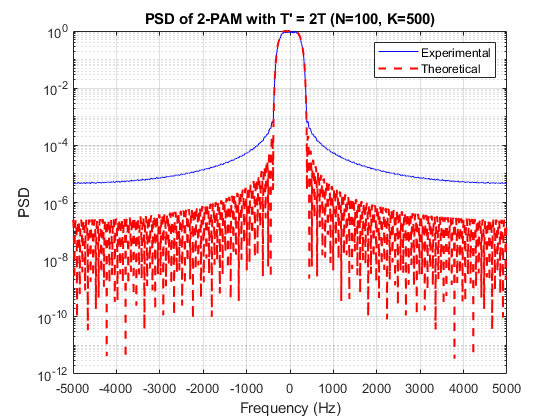
\includegraphics[width=0.7\textwidth]{A5.png}
    \caption{PSD with $T' = 2T$ showing narrower bandwidth.}
    \label{fig:a5_psd}
\end{figure}

\subsection*{A.6 Design Decisions}
\begin{itemize}
    \item To transmit data as fast as possible in the same bandwidth, we choose \textbf{4-PAM} because it carries 2 bits/symbol compared to 1 bit/symbol for 2-PAM.
    \item If bandwidth is expensive, we choose \textbf{$T' = 2T$} (or larger), as it reduces the spectral footprint.
\end{itemize}

\section*{Part B: Stochastic Processes}

Let $Y(t) = X \cos(2\pi F_0 t + \Phi)$ with $X \sim N(0,1)$ and $\Phi \sim U[0, 2\pi]$.

\subsection*{B.1 Realizations}
Five realizations of the process are shown below.

\begin{figure}[H]
    \centering
    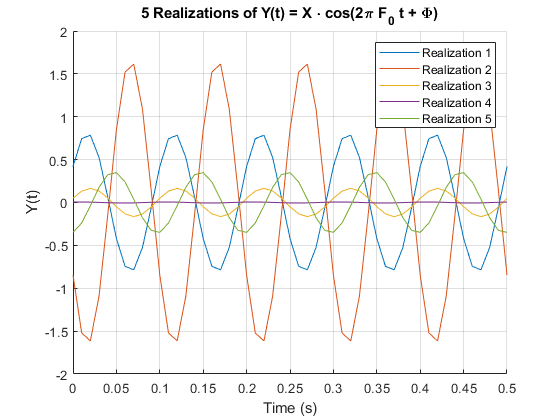
\includegraphics[width=0.7\textwidth]{B1.png}
    \caption{5 realizations of the stochastic process $Y(t)$.}
    \label{fig:b1}
\end{figure}

\subsection*{B.2 Mean and Autocorrelation}
\textbf{Mean:}
\[ E[Y(t)] = E[X \cos(2\pi F_0 t + \Phi)] = E[X] E[\cos(2\pi F_0 t + \Phi)] = 0 \cdot E[\dots] = 0 \]

\textbf{Autocorrelation:}
\[ R_{YY}(t+\tau, t) = E[Y(t+\tau)Y(t)] = E[X^2 \cos(2\pi F_0(t+\tau) + \Phi) \cos(2\pi F_0 t + \Phi)] \]
Using the identity $\cos A \cos B = \frac{1}{2}[\cos(A-B) + \cos(A+B)]$:
\[ R_{YY}(\tau, t) = \frac{1}{2} E[X^2] \{ \cos(2\pi F_0 \tau) + E[\cos(2\pi F_0(2t+\tau) + 2\Phi)] \} \]
Since $E[X^2] = 1$ and $E[\cos(\dots + 2\Phi)] = 0$:
\[ R_{YY}(\tau) = \frac{1}{2} \cos(2\pi F_0 \tau) \]
The process is \textbf{Wide-Sense Stationary (WSS)} because its mean is constant and its autocorrelation depends only on $\tau$.

\subsection*{B.3 Power Spectral Density}
The PSD $S_Y(F)$ is the Fourier Transform of $R_{YY}(\tau)$:
\[ S_Y(F) = \mathcal{F}\left\{ \frac{1}{2} \cos(2\pi F_0 \tau) \right\} = \frac{1}{4} [\delta(F - F_0) + \delta(F + F_0)] \]

\end{document}
